\documentclass[10pt,a4paper,oneside]{report}
\usepackage{graphicx}
\usepackage{lscape}
\begin{document}
\title{Group 7 Integrated Project Proposal}
\author{Will Hua\\
        Jon Playdon\\
        Alex Remedios\\
        Robert Harmer\\
        Douglas McIntyre\\
        Mateusz Kowalczyk}
%\date{}
\maketitle
\section*{Alex}

The mobile app market is one of the newest and fastest growing parts of the software industry. Since the popularisation of smartphones, the ability to produce third party applications has led to a brand new platform for utilities, entertainment, education and communication which did not exist a few years ago. From freely available programs which turn your phone into a torch, to fully fledged simulation games which only existed on games consoles, apps have appeared in every shape and form.\\


The key to a successful app, is providing a service using robust software with a comfortable and consistent interface. Our idea is to create a turn based game which users can play against AI, against each other locally, or against each other across a network. The platform will be the android operating system. There are many reasons for this decision; primarily, we believe that the turn based game is perfect for mobile platforms and it’s potential has not been fulfilled. The closest we have come to a wildly popular turn based game for smartphone is ‘draw something’, which demonstrated how less can be more when it comes to mobile gameplay. With simple yet attractive graphics, and easily recognisable short and long term game objectives, we hope *our game* will become our go-to game whenever we have a moment to spare.\\
We will take advantages of all the unique features of the mobile platform by designing a game which is easy to ‘pick up and play’, uses a touch interface, has a strong social aspect, and is free.\\


Originally made for business use, the smartphone has become overwhelmingly popular in the 13-25 age bracket, which is the demographic our app will be aiming for. Combining a mixture of battle play (reminiscent of Advanced Wars), and competition with friends, we hope to satisfy both ends of this range. Whilst our game will be simple, we intend to promote an element of strategy, stemming from ground rules and unit constraints, in the same way chess does. This will make *our game* stimulating and difficult to put down.\\


Whilst our idea is by no means unique, there is a lack of currently popular games like the one we intend to make. A new turn based game would be refreshing compared to the currently popular single-player arcade style games like Angry Birds.
\clearpage
\section*{Jon}
\clearpage
\section*{Doug}
\clearpage
\section*{Rob}
\clearpage
\section*{Kowal - Collaboration}

Our project will be a collaborative effort of multiple group members working separately on different parts of the system which will then come together to form a finished product. In order to be able to combine parts of the system together into a working entity, all group members need to know what other members are doing. This section isn`t about the interface that will be established during the design stage of the project that we will be able to use to make sure that each part of the system will be able to communicate with another. This section is about collaborating as a team towards a single goal and being able to see and possibly change each others' work, as well as to prevent overwriting each others' work. This is mainly applicable to the programming stage of the project as that's where it is most likely that a member might be wanting to make a change that other members have to be able to see. \\


The solution we have decided to use is the git version control system. Git allows every single member of the group to work on the system locally, making incremental changes. When ready, a group member can push the changes into an online code repository where other group members will be able to see them. The strength of git is the ability to detect when code conflicts occur. If both members change the same part of code, they will be prevented from overwriting the new code without resolving the issue. Furthermore, all users have a copy of the code and can work on it at any time, meaning that they don't have to have network access until the stage where they want to submit the code. Git also features ``branches'' which allow people to work on now concepts or ideas without affecting the main development. As in any version control system, the users are able to roll back the changes to any point in time, meaning that any blunders can be easily reversed. On top of this ability, git is able to make powerful partial reverts, meaning that not all work is lost if we only want to roll back a part of the system. All commits to the system are signed with the commiters name and e-mail address meanining that it's trivial pinpoint who made what changes to the code base.\\

\
As far as the non-programming part of the project goes, regular meetings will be held where group members can discuss any issues they might me having, or any changes they want to make. The work will be split into multiple parts at the beginning of the development life cycle, and those meetings are there to ensure that everyone is keeping up with their work load.\\

All group members have other members' contact details, so we are able to contact any member of the team on individual basis if at all required. We believe that the combination of regular meetings where we can review the progress and the use of a version control system where everyone can see the code is enough to keep the team working efficiently.

\begin{landscape}
\begin{center}
\hspace*{-1.5in}
\vspace*{-1.5in}
\section*{Will}
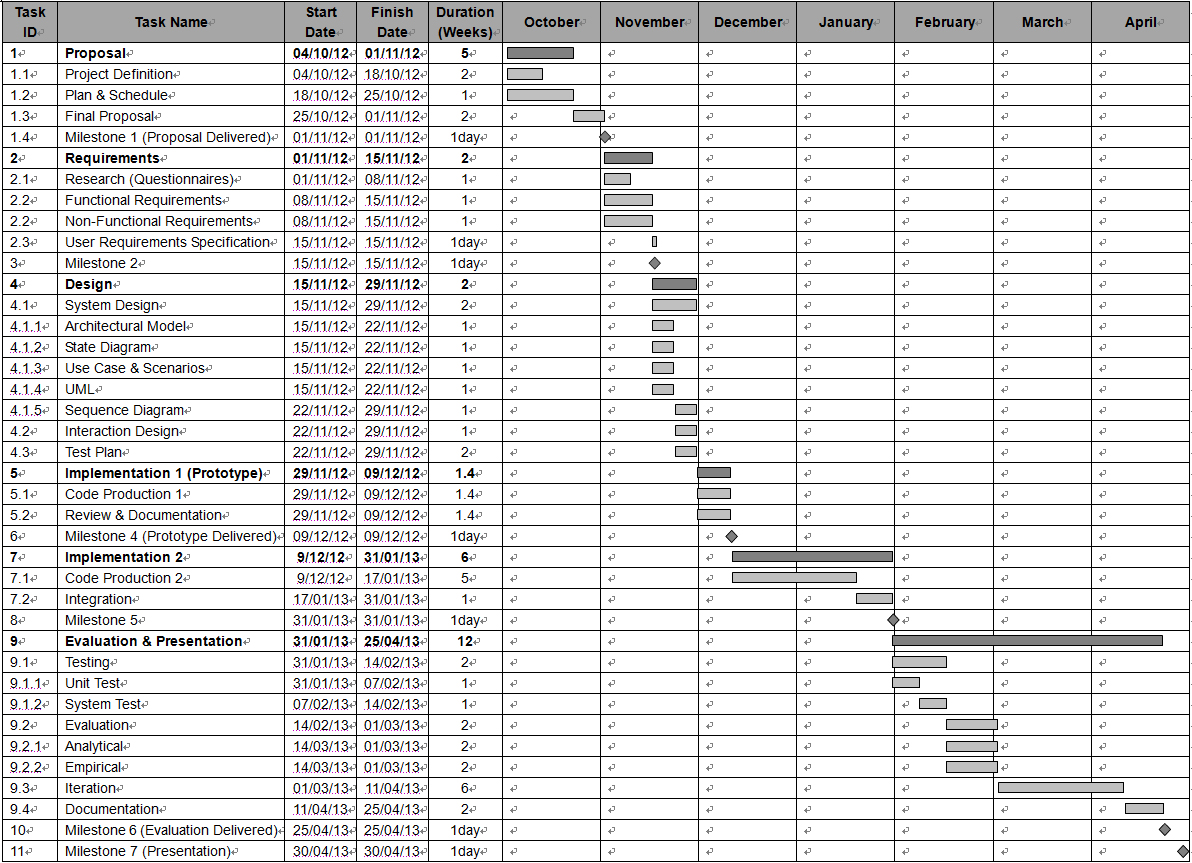
\includegraphics[height=\textheight,keepaspectratio]{gantt.jpg}
\end{center}
\end{landscape}
\end{document}
